\documentclass[main.tex]{subfiles}
\begin{document}
\section{Vector Analysis in $\reals^n$}
\subsection{$\reals^3$ Case}
We will try to give quite precise but still a heuristic formulation of the Stokes's Theorem in $\reals^3$ case, which is a ceratin compromise between being realitive easy to comprehend and rigorous enough to be comfortably used in most physical applications. The serious mathematical treatment of Stokes theorem for differentiable manifolds can be found in  e.g. \cite{spivak1995} or \cite{warner1983}. However, in my opinion, it is propedeutically recommended to understand first the $\reals^3$ case in a heuristic way, as presented here, to be ready for more advanced and rigorous treatment of this topic in differentiable manifolds theory. 
\begin{definition}
\label{orientation-2d}
We say that the picewise smooth surface $(S, \vec{n})$ is oriented when $\vec{n}:S\to \reals^3$ is a picewise $C^1$ continous field of normed vectors perpendicular to $S$ in each point.  
\end{definition}
\begin{definition}
\label{orientation-1d}
We say that the piecewise smooth curve $(\Gamma, \vec{l})$ is oriented when $\vec{l}:\Gamma\to\reals^3$ is a picewise $C^1$ field of normed vectors tanget to $\Gamma$ in each point.
\end{definition}
\begin{definition}
\label{consistent-orientation-2d}
Let $(S,\vec{n})$ be an oriented surface and let $\Gamma \subset \partial S$ be a picewise smooth closed oriented curve $(\Gamma, \vec{l})$. We say that these orientations are consistent if $\vec{n}\times \vec{l}$ is directed towards $S$ for any point of $\Gamma$.
\end{definition}
\begin{theorem} (\textbf{Stokes's Theorem})
Let $(S, \vec{n})$ be a bounded, picewise smooth, oriented surface in $\reals^3$. Let $(\partial S, \vec{l})$ be a picewise $C^1$ edge-boundary of $S$ consisting of finitelly many closed curves oriented consistently with $S$. Let $\Omega$ be on open set such that $S\subset \Omega$. Let $ds$ symbolise an infinitesimal element of $\partial S$ and $dS$ an infinitesimal element of surface $S$. If $\vec{F}\in C^1(\Omega, \reals^3)$, then
\begin{equation}
\oint_{\partial S} \vec{F} \cdot (ds)\vec{l} = \int_S (\nabla \times \vec{F}) \cdot (dS)\vec{n}.
\end{equation}
\end{theorem}
\begin{figure}[H]
\centering
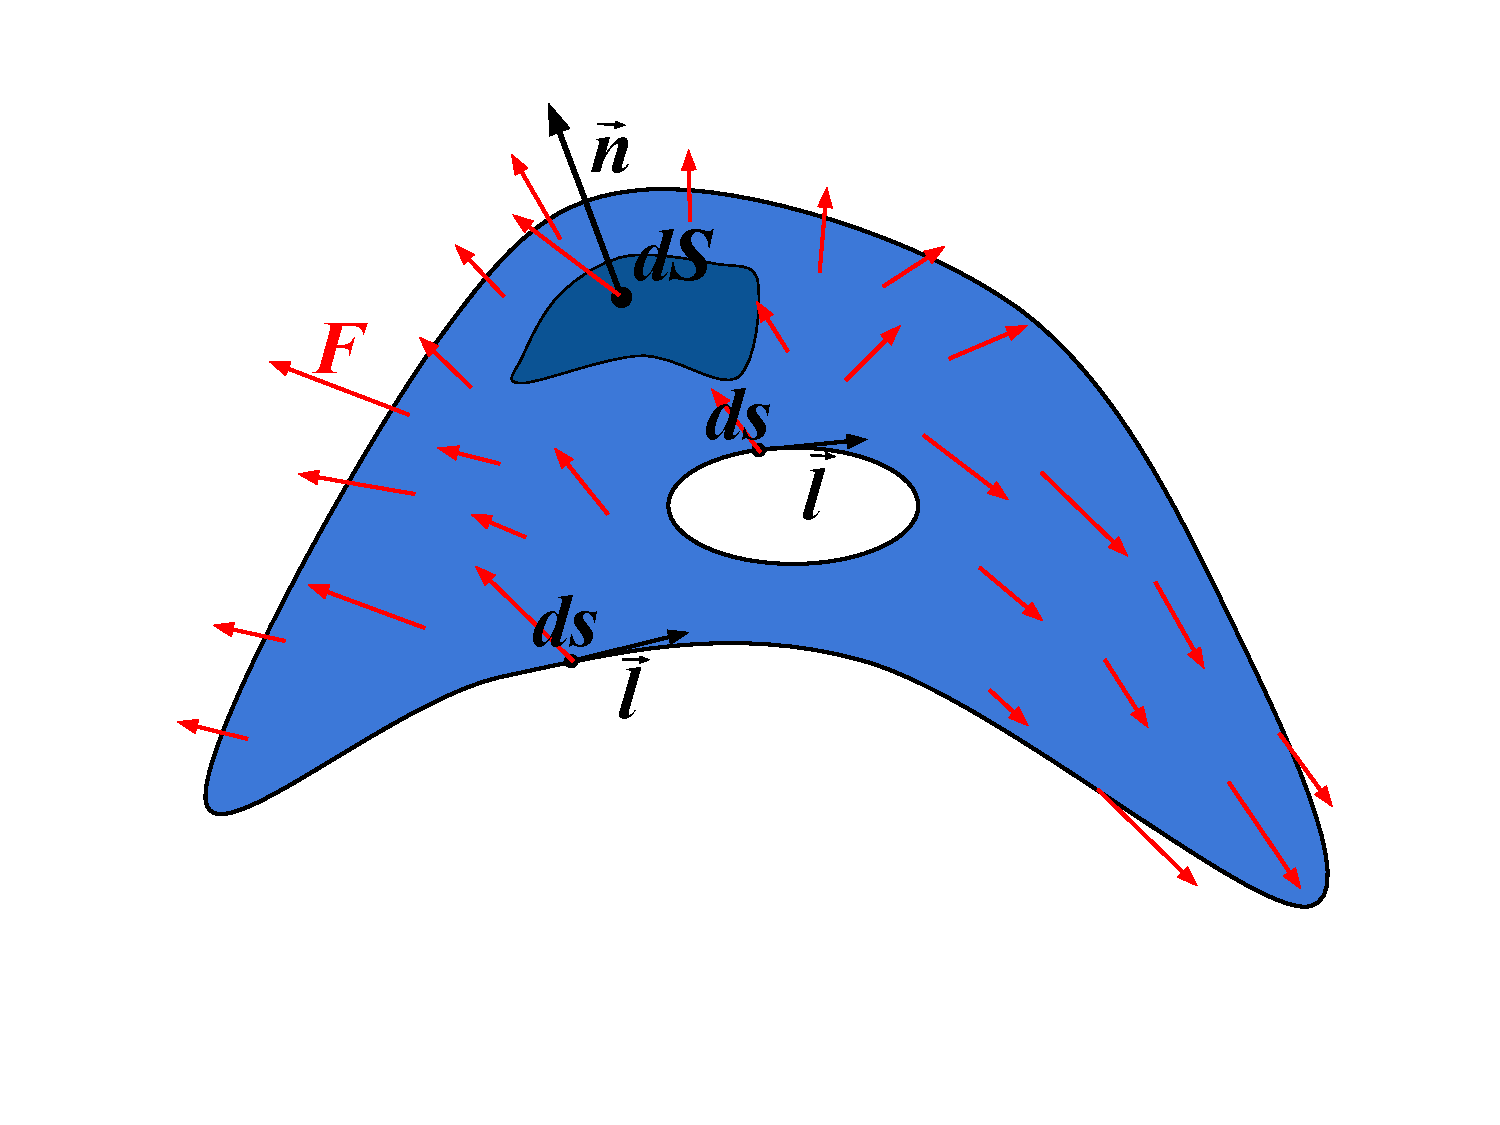
\includegraphics[scale=0.5]{figs/Stokes}
\caption{Ilustration for Stokes Theorem}
\end{figure}
\begin{proof}
\cite[see][7.3 Stokes’s and Gauss’s Theorems]{colley2012}
\end{proof}
\begin{theorem}(\textbf{Gauss's Theorem})
Let $\Omega$ be an open an connected subset of $\reals^3$. Let $(\partial \Omega, \vec{n})$ be a picewise smooth directed closed surface, such that $\vec{n}$ points outside $\Omega$. Let $dV$ symbolise an infinitesimal element of volume $\Omega$ and let $dS$ symbolise an infinitesimal element of surface $\partial \Omega$. If $\vec{F}\in C^1(\text{Clo}(\Omega), \reals^3)$, then
\begin{equation}
\oint_{\partial\Omega} \vec{F} \cdot (dS)\vec{n} = \int_\Omega \nabla \cdot \vec{F} dV.
\end{equation} 
\end{theorem}
\begin{proof}
\cite[see][7.3 Stokes’s and Gauss’s Theorems]{colley2012}
\end{proof}
\subsection{Introduction to Differential Forms on Manifolds Embedded in Real Coordinate Space}
\label{simplified-manifolds}
In this subsection we will consider only parametrised smooth manifolds with one map. This is an obvious simplification, but we will treat this only as a traning before doing serious differentiable manifolds theory. This is a propedeutical way taken after \cite{colley2012} with only slight modifications.
We will first introduce a concept of differentiable $k$-form.
\begin{definition}
A basis $k$-form in $\reals^n$
\begin{equation}
dx_{i_1}\form\dots\form dx_{i_k},
\end{equation}
where $i_1, \dots, i_k = 1,\dots, n$,
is a multi-linear function from $\reals^n$ to $\reals$ such that 
\begin{equation}
dx_{i_1}\form\dots\form dx_{i_k}(\vec{a_1}, \dots, \vec{a_k}) := 
\det\begin{bmatrix}
dx_{i_1}(\vec{a_1}) & \dots & dx_{i_1}(\vec{a_k}) \\
\vdots & \ddots & \vdots \\
dx_{i_k}(\vec{a_1}) & \dots & dx_{i_k}(\vec{a_k})
\end{bmatrix}
\end{equation}
where for $\vec{a} = [a_1, \dots, a_n]$, $dx_j(\vec{a}) = a_j$.
\end{definition}
\begin{definition}
Let $U$ be an open subset of $\reals^n$. A differentiable $k$-form on $U$
\begin{equation}
\omega(x) = \sum_{i_1, \dots, i_k} F_{i_1, \dots, i_k}(x) dx_{i_1}\form\dots\form dx_{i_k}
\end{equation}
is a mapping from $U$ to the space of multi-linear functions from $\reals^n$ to $\reals$, where $F_{i_1, \dots, i_k}\in C^1(U)$ and 
\begin{equation}
\omega(x)(\vec{a_1}, \dots, \vec{a_k}) = \sum_{i_1, \dots, i_k} F_{i_1, \dots, i_k} (x) dx_{i_1}\form\dots\form dx_{i_k}(\vec{a_1}, \dots, \vec{a_k}).
\end{equation}
A differentiable $0$-form is each function from $C^1(U, \reals)$. For formal reasons we assume that basis $0$-form is constant function $=1$.
\end{definition}
We treat $\form$ as a natural operator on basis forms with assumed associativity.
It follows from the definition of determinant that if any $dx_i$ appears twice the basis form is equal to $0$ and it changes sign when we swap two of its elements.
\begin{definition}
Let $\omega_1 = \sum_i f^1_i \Omega^1_i$ be a differentiable $k$-form and $\omega_2 = \sum_j f^2_j \Omega^2_j$ be a differentiable $l$-form where $\Omega^1_i$ are basis $k$-forms and $\Omega^2_j$ are basis $l$-forms.
\begin{equation}
\omega_1 \form \omega_2 :=  \sum_i \sum_j f^1_i f^2_j (\Omega^1_i \form \Omega^2_j).
\end{equation}
\end{definition}
\begin{theorem}
Let $\omega, \omega_1, \omega_2$ be differentiable $k$-forms, $\nu$ be differentiable $l$-form and $\tau$ be a $p$-form. Let $f$ be $0$-form Then
\begin{enumerate}
\item $(\omega_1 + \omega_2)\form \nu = \omega_1\form \nu + \omega_2\form \nu$.
\item $\omega\form \nu = (-1)^{kl}\nu\form\omega$.
\item $(\omega\form \nu) \form p = \omega\form(\nu\form p)$.
\item $(f\omega)\form \nu = f(\omega\form \nu) = \omega\form (f\nu)$. 
\end{enumerate}
\end{theorem}
\begin{definition}
Let $\omega = \sum_j f_j \Omega_j$ be a differentiable $k$-form on $U\subset\reals^n$ where $\Omega_i$ are basis $k$-forms.
\begin{equation}
d\omega := \sum_j \sum_{i=1}^n \cfrac{\partial f_j}{\partial x_i} dx_i \form \Omega_j. 
\end{equation}
\end{definition}
Now we will introduce a simplified concept of manifold.
\begin{definition}
Let $D\subset \reals^k$ be a region consists of some open set $U$ and any parts of its clousure.
$X$ is parametrised $k$-manifold if
$X:D\to \reals^n$ and
\begin{enumerate}
\item
$X|_U$ is 1-to-1 and $C^1$ class.
\item
$\frac{\partial X}{\partial u_1}, \dots, \frac{\partial X}{\partial u_k}$ are linearly independent.
\end{enumerate}
\end{definition}
\begin{definition}
Let $X$ be a parametrised $k$-manifold.
\begin{equation}
T^i_X := \cfrac{\partial X}{\partial u_i}.
\end{equation}
We say that $T^i_X$ is a tangent vector to $i$-th coordinate curve. 
\end{definition}
\begin{definition}
\label{simple-manifold-orientation}
Let $X$ be parametrised $k$-manifold. $k$-form $\Omega$ is called an orientation of $X$, iff
\begin{equation}
\Omega(T_X^1, \dots, T_X^k) > 0.
\end{equation}
at each point of $X$.
\end{definition}
\begin{proposition}
Let $\vec{a}, \vec{b}, \vec{c}\in \reals^3$, then
\begin{equation}
\det(\vec{a}, \vec{b}, \vec{c}) = \vec{a}\cdot (\vec{b}\times \vec{c}).
\end{equation} 
\end{proposition}
\begin{example}
\label{surface-orientation}
Let $X$ be a parametrised $2$-manifold and
\begin{equation} 
\vec{n} = \cfrac{T^1_X\times T^2_X}{\norm{T^1_X\times T^2_X}}. 
\end{equation}
Note that $(X,\vec{n})$ is an orientation of $X$ in terms of Definition \ref{orientation-2d}. Indeed $\vec{n}$ is a unit vector perpendicular to the tanget space. The corresponding orientation in terms of Definition \ref{simple-manifold-orientation} is 
\begin{equation}
\Omega(\vec{a}^1, \vec{a}^2) = \det(\vec{n}, \vec{a}^1, \vec{a}^2).
\end{equation}
\end{example}
\begin{proof}
Note that $\Omega(T^1_X, T^2_X) > 0$ because
\begin{equation}
\Omega(T^1_X, T^2_X) = \cfrac{1}{\norm{T^1_X\times T^2_X}}(T^1_X\times T^2_X)\cdot (T^1_X\times T^2_X) > 0.
\end{equation}
\end{proof}
\begin{definition}
\label{simple-induced-orientation}
Let $X$ be a parametrised $k$-manifold and $Y$ be a parametrised $k-1$-manifold such that $Y$ is contained in a boundary of $X$. Let $\Omega_X$ be an orientation of $X$. We say that orientation of $Y$ is induced by orientation of $X$ iff
\begin{equation}
\Omega_Y(\vec{a}^1, \dots, \vec{a}^{k-1}) := \Omega(\vec{v}, \vec{a}^1, \dots, \vec{a}^{k-1}) 
\end{equation}
is an orientation of $Y$ where $\vec{v}$ is a vector field on $X$ such that $\vec{v}$ is tangent to $X$ (i.e. is a linear combination of $T_X^1, \dots, T_X^k$), normal to $Y$ (i.e. perpendicular to each $T_Y^1, \dots, T_Y^{k-1}$) and $-\vec{v}$ on $Y$ points towards $X$.
\end{definition}

\begin{proposition}
Induced orientation from Definition \ref{simple-induced-orientation} coincides with consistent orientation from Definition \ref{consistent-orientation-2d}
\end{proposition}
\begin{proof}
Let $X$ be parametrised $2$-manifold. Let
\begin{equation}
\vec{n} := \cfrac{T^1_X\times T^2_X}{\norm{T^1_X\times T^2_X}}.
\end{equation}
As it was previously noted, $(X,\vec{n})$ is an orientation of $X$ in terms of Definition \ref{orientation-2d}.
We have shown in Example \ref{surface-orientation} that $\Omega_X(\vec{a}^1, \vec{a}^2) = \det(\vec{n}, \vec{a}^1, \vec{a}^2)$ is orientation of $X$ in terms of Definition \ref{simple-manifold-orientation}.
Let $Y$ be a parametrised $1$-manifold (i.e. curve) such that $Y$ is contained in a boundary of $X$. Let
\begin{equation}
\vec{l} := \cfrac{T_Y^1}{\norm{T_Y^1}}.
\end{equation}
Note that $\vec{l}$ is a unit vector tangent to $Y$ at each point. Thus $(Y, \vec{l})$ is an orientation of $Y$ in terms of Definition \ref{orientation-1d}.

Let $\vec{v}$ be some vector filed on $Y$ wich is tangent to $X$ and perpendicular to $Y$ and $-\vec{v}$ points towards $X$.   
\begin{equation}
\Omega(\vec{a}) := \Omega_X(\vec{v}, \vec{a}) = \det(\vec{n}, \vec{v}, \vec{a}) = \vec{n}\cdot (\vec{v}\times \vec{a}) = \vec{v}\cdot(\vec{a}\times \vec{n}).
\end{equation}
$\Omega$ is obviously a good candidate for orientation of $Y$. Now all we need to do is to check the sign of $\Omega(\vec{l})$.
\begin{equation}
\Omega(\vec{l}) = \vec{v}\cdot(\vec{l}\times \vec{n}) = -\vec{v}\cdot(\vec{n}\times\vec{l}).
\end{equation}

Notice that because $\vec{v}$ is tangent to $X$ and perpendicular to $Y$, we have $-\vec{v} \parallel \vec{n}\times \vec{l}$. Thus, $\Omega(\vec{l}) > 0$ if and only if $\vec{n}\times \vec{l}$ points in the same direction as $-\vec{v}$, i.e. towards $X$. And this means that $\Omega$ is an orientation of $Y$ induced by $X$ if and only if orientation $(Y,\vec{l})$ is consistent with orientation $(X, \vec{n})$ in terms of Definition \ref{consistent-orientation-2d}.
\end{proof}
\begin{definition}
Let $X: D\to \R^n$ be parametrised $k$-manifold. Let $\omega$ be a $C^1$ $k$-form defined on an open set $U$ such that $X(D)\subset U$.
\begin{equation}
\int_X \omega := \int_D \omega(T_X^1, \dots, T_X^k)du,
\end{equation}
where $du$ symbolise an infinitesimal volume element of $D$.  
\end{definition}
The central theorem in this section is Stokes's Theorem.
\begin{theorem}(\textbf{Stokes's Theorem})
\label{par-manifold-stokes}
Let $X: D\to \R^n$ be parametrised $k$-manifold. Let $\partial X$ be $k-1$-manifold which image is equal to the boundary of $X$. Let $\omega$ be a $C^1$ $k$-form defined on an open set $U$ such that $X(D)\subset U$. If orientation of $\partial X$ is induced by $X$, then
\begin{equation}
\int_{X} d\omega = \int_{\partial X} \omega.
\end{equation}
\begin{lemma}
\label{surface-element}
Let $X:D\to\reals^3$ be a parametrised $2$-manifold. Let $du$ be an infinitesimal element of $D$. Let $dS = X(du)$ be a corresponding infinitesimal surface element of $X$. Then
\begin{equation}
dS = \norm{T^1_X\times T^2_X}du.
\end{equation}
\end{lemma}
\begin{proof}
Let $u = (u_1, u_2)$ and $\Delta u = (\Delta u_1, \Delta u_2)$ with $\Delta u_1, \Delta u_2$ being infinitesimals of the first order. Imagine an infinitesimal volume element $du$ as $[u_1, u_1 + \Delta u_1]\times [u_2, u_2 + \Delta u_2]$. Let $\theta = (\theta_1, \theta_2)$ Neglecting second-order infinitesimals we have
\begin{equation}
X(u + \theta\cdot\Delta u) = X(u) + 
\begin{bmatrix}
\cfrac{\partial X}{\partial u_1} & \cfrac{\partial X}{\partial u_2}
\end{bmatrix}
\begin{bmatrix}
\theta_1\Delta u_1 \\
\theta_2\Delta u_2
\end{bmatrix} 
= X(u) + \theta_1\Delta u_1 T_X^1 + \theta_2\Delta u_2 T_X^2.
\end{equation}
Note that
\begin{equation}
du = \mu([u_1, u_1 + \Delta u_1]\times [u_2, u_2 + \Delta u_2]) = \mu\{\theta\cdot\Delta u:\theta\in[0,1]^2\}.
\end{equation}
Thus
\begin{equation}
dS = X(du) = \mu\{\theta_1\Delta u_1 T_X^1 + \theta_2\Delta u_2 T_X^2:\theta\in[0,1]^2\}.
\end{equation}
But this equal to the area of the parallelogram spanned by $\Delta u_1 T_X^1$ and $\Delta u_2 T_X^2$, which is equal to $\norm{T^1_X\times T^2_X}\Delta u_1\Delta u_2 = \norm{T^1_X\times T^2_X}du$.
\end{proof}
\begin{example}
\label{form2normal-surface}
Let $X$ be a parametrised $2$-manifold. Let $\vec{n} = \cfrac{T^1_X\times T^2_X}{\norm{T^1_X\times T^2_X}}$. Let $F=[F^1, F^2, F^3]\in C^1(U, \reals^3)$, where $X\subset U$. Let 
\begin{equation}
\omega = F^1 dx_2 \form dx_3 + F^2 dx_3\form dx_1 + F^3 dx_1\form dx_2. 
\end{equation}
Then
\begin{equation}
\int_X  \omega = \int_X
\begin{bmatrix}
F^1 & F^2 & F^3
\end{bmatrix} \cdot \vec{n} dS.
\end{equation}
\end{example}
\begin{proof}
\begin{multline}
\omega(T^1_X, T^2_X) = F^1 dx_2 \form dx_3(T^1_X, T^2_X) + \dots = 
F_1
\begin{vmatrix}
dx_2(T_X^1) & dx_2(T_X^2) \\
dx_3(T_X^1) & dx_3(T_X^2) \\  
\end{vmatrix} + \dots = \\
\begin{bmatrix}
F^1 & F^2 & F^3
\end{bmatrix} \cdot (T_X^1\times T_X^2) = 
\begin{bmatrix}
F^1 & F^2 & F^3
\end{bmatrix} \cdot \vec{n} \norm{T_X^1\times T_X^2} 
\end{multline}
Thus by Lemma \ref{surface-element} we have
\begin{equation}
\int_X  \omega = \int_D \begin{bmatrix}
F^1 & F^2 & F^3
\end{bmatrix} \cdot \vec{n} \norm{T_X^1\times T_X^2} du
= \int_X 
\begin{bmatrix}
F^1 & F^2 & F^3
\end{bmatrix} \cdot \vec{n} dS.
\end{equation}
\end{proof}
\end{theorem}

\begin{theorem}
\label{gauss-theorem-multidimensional}
(\textbf{Gauss's Theorem $n$-dimensional case})
\label{n-gauss-thoerem}
Let $\Omega$ be an open an connected subset of $\reals^n$. Let $\vec{n}$ be a fector field of unit vectors, normal to a picewise smooth closed surface of $\partial \Omega$, such that $\vec{n}$ points outside $\Omega$. Let $dV$ symbolise an infinitesimal element of $n$-dimentional volume of $\Omega$ and let $dS$ symbolise an infinitesimal element of surface $\partial \Omega$. If $\vec{F}\in C^1(\text{Clo}(\Omega), \reals^n)$, then
\begin{equation}
\oint_{\partial\Omega} \vec{F} \cdot (dS)\vec{n} = \int_\Omega \nabla \cdot \vec{F} dV.
\end{equation} 
\end{theorem}
\begin{proof}
Follows from Theorem \ref{par-manifold-stokes} (Stokes's Theorem).
\end{proof}   
\section{Group Theory}
\subsection{Generators}
In this subsection we will use Einstein summation convention.
Let's assume we have certain continous symetry $u_{(\epsilon)}(x)$ of $\reals^n$ with a generator $g$ (i.e. $\cfrac{du_{\epsilon}}{d\epsilon}\bigg\vert_{\epsilon=0} = g$). This symetry on domain induce a transformation of functions.
\begin{equation}
f \mapsto f\circ u_{(\epsilon)}
\end{equation}
We will show that the generator of this transformation (at least in a pointwise sense) is 
\begin{equation}
f\mapsto\nabla f \cdot g.
\end{equation}
We would like to calculate $\cfrac{d(f\circ u_{(\epsilon)})}{d\epsilon}\bigg\vert_{\epsilon=0}$.
\begin{equation}
\cfrac{d(f\circ u_{(\epsilon)})}{d\epsilon} \bigg\vert_{\epsilon=0}= \cfrac{\partial f}{\partial x^i}\cfrac{du_{(\epsilon)}^i}{d\epsilon}\bigg\vert_{\epsilon=0} = \nabla f \cdot g.
\end{equation}
Although it is not shown here, it seems it could be changed into a rigorous theorem, that if we consider the space $L^2(\reals^n)$, the convergence in deriviative above is in $L^2$ norm sense.
\begin{example}
Consider one dimensional case. Let $u_{(\epsilon)}(x) = x + \epsilon$. In this case generator of $u_{(\epsilon)}$ is just $1$. Thus the generator of $f \mapsto f\circ u_{(\epsilon)}$ is $\cfrac{d}{dx}$.
\end{example}

\begin{example}
Rotation on plane.
Let
\begin{equation}
u_{(\theta)}(x) = 
\begin{bmatrix}
\cos\theta & -\sin\theta \\
\sin\theta & \cos\theta \\
\end{bmatrix}
\begin{bmatrix}
x^1 \\
x^2
\end{bmatrix}.
\end{equation}
The generator of $f \mapsto f\circ u_{(\theta)}$ is 
\begin{equation}
x^1\cfrac{\partial}{\partial x^2} - x^2 \cfrac{\partial}{\partial x^1}.
\end{equation}
\end{example}
\begin{proof}
\begin{equation}
g(x) = \begin{bmatrix}
0 & -1 \\
1 & 0 \\
\end{bmatrix}
\begin{bmatrix}
x^1 \\
x^2
\end{bmatrix}
= 
\begin{bmatrix}
-x^2 \\
x^1
\end{bmatrix},
\end{equation}
thus
\begin{equation}
\nabla f(x) \cdot g(x) = 
\begin{bmatrix}
\cfrac{\partial f}{\partial x^1} & \cfrac{\partial f}{\partial x^2}
\end{bmatrix}
\begin{bmatrix}
-x^2 \\
x^1
\end{bmatrix}
= x^1 \cfrac{\partial f}{\partial x^2} - x^2 \cfrac{\partial f}{\partial x^1}.
\end{equation}
\end{proof}
\begin{proposition}
If $u_{(\theta)}$ is a rotation about an axis specified by unit vector $n$ with an angle $\theta$ measured couterclockwise if seen from the tip of $n$, then
\begin{equation}
\cfrac{du_{(\theta)}(x)}{d\theta}\bigg\vert_{\theta=0}=n\times x.
\end{equation} 
\end{proposition}
\begin{proof}
Choose an orthonormal basis $n$, $a$, $b$ (hint: they corespond to $x,y,z$ respectively in stanard setup) such that
\begin{equation}
\label{right-hand-rel-in-basis}
a \times n = -b \text{ and } b \times n = a.
\end{equation}
Then
\begin{multline}
u_{(\epsilon)}(x) = (u\cdot x)u + \\
((a\cdot x)\cos\theta - (b\cdot x)\sin\theta)a
+ ((a\cdot x)\sin\theta + (b\cdot x)\cos\theta)b.
\end{multline}
Thus
\begin{equation}
\cfrac{du_{(\theta)}(x)}{d\theta}\bigg\vert_{\theta=0} 
= -(b\cdot x)a + (a\cdot x)b.
\end{equation}
We will show that 
\begin{equation}
\label{rot-gen-rep}
n\times x = -(b\cdot x)a + (a\cdot x)b.
\end{equation}
It's obvious that
\begin{equation}
n\cdot(n\times x) = 0.
\end{equation}
By Theorem \ref{inner-cross} and (\ref{right-hand-rel-in-basis}), we have
\begin{equation}
a\cdot(n\times x) = x\cdot(a\times n) = -x \cdot b.
\end{equation}
and
\begin{equation}
b\cdot(n\times x) = x\cdot(b\times n) = x \cdot a.
\end{equation}
The 3 equations above are equivalent to (\ref{rot-gen-rep}), which completes the proof.
\end{proof}
\begin{example}
Rotation in $\reals^3$.
Let $u_{(\theta)}$ be a rotation about an axis specified by unit vector $n$ with an angle $\theta$ measured couterclockwise if seen from the tip of $n$. The generator of $f \mapsto f\circ u_{(\theta)}$ is
\begin{equation}
\label{rot-gen}
f\mapsto n\cdot(x\times \nabla f).
\end{equation}
\end{example}  
\begin{proof}
Note that by Theorem \ref{inner-cross} $\nabla f \cdot (n\times x) =
n\cdot(x\times \nabla f)$.
\end{proof}
For the benefit of the reader, let's write explicitly generator from (\ref{rot-gen}):
\begin{equation}
n\cdot\bigg(x^2\cfrac{\partial}{\partial x^3} - x^3\cfrac{\partial}{\partial x^2},\; x^3\cfrac{\partial}{\partial x^1} - x^1\cfrac{\partial}{\partial x^3},\; x^1\cfrac{\partial}{\partial x^2} - x^2\cfrac{\partial}{\partial x^1}\bigg).
\end{equation}
\section{Tensor Analysis}
\subsection{Vectors and dual vectors}

Let $V$ be a vector space and $V^*$ be a dual space to the $V$. Let $\{e_i\}$ be an arbitrary base of $V$. $\{e^i\}\subset V^*$ is a dual base to $\{e_i\}$ iff

\begin{equation}
\boxed{e^i(e_j) = \delta^i_j}
\end{equation}

\noindent
Let $\{\hat{e}_i\}$ be another base of $V$ and $\{\hat{e}^i\}$ be its dual base. We have two transition matrices
$[X^i_{\hat{j}}]$ and $[X^{\hat{i}}_{j}]$ such as

\begin{equation}
\label{con_trans}
\hat{e}_k = \sum_i X^i_{\hat{k}}e_i,
\end{equation}

\begin{equation}
\hat{e}^k = \sum_i X^{\hat{k}}_i e^i.
\end{equation}

\begin{fact}
$\sum_i X^l_{\hat{i}}X^{\hat{i}}_k = \delta^l_k.$
\end{fact}
\begin{proof}
$\delta^l_k = \hat{e}^l(\hat{e}_k) = (\sum_i X^{\hat{l}}_i e^i)(\sum_j X^j_{\hat{k}}e_j) = 
\sum_i\sum_j X^{\hat{l}}_i X^j_{\hat{k}} e^i(e_j)$

$= \sum_i\sum_j X^{\hat{l}}_i X^j_{\hat{k}} \delta^i_j = \sum_i X^{\hat{l}}_i X^i_{\hat{k}}.$
\end{proof}
\begin{corollary}
$$
e_j = \sum_k X^{\hat{k}}_j \hat{e}_k,
$$

$$
e^j = \sum_k X^j_{\hat{k}} \hat{e}^k.
$$
\end{corollary}

\begin{corollary}
If $\sum_j v^j e_j = \sum_j \hat{v}^j \hat{e}_j$ then $\hat{v}^k = \sum_j X^{\hat{k}}_j v^j$.
\end{corollary}

\begin{corollary}
If $\sum_j v_j e^j = \sum_j \hat{v}_j \hat{e}^j$ then $\hat{v}_k = \sum_j X^j_{\hat{k}} v_j$.
\end{corollary}

\subsection{Tensors} 
\begin{definition}
A tensor of type $\binom{m}{n}$ is a multilinear function $T:(V^*)^m \times V^n \to \R$.
\end{definition}

\noindent
Let $\mathcal{T}\binom{m}{n}$ be a space of all tensors of the type $\binom{m}{n}$. It is trivial to notice that $\mathcal{T}\binom{m}{n}$ is a vector space.

Note that $\mathcal{T}\binom{0}{1} = V^*$. And as we can define for $v\in V$ and $w^*\in V^*$, $v(w^*) := w^*(v)$, we will identify $V$ with $\mathcal{T}\binom{1}{0}$.

Notice that because of multilinearity tensor is uniquely defined by the set of numbers $\{T^{\mu_1\dots\mu_m}_{\nu_1\dots\nu_n}\}$, where
\begin{equation}
\label{ten_coef}
T^{\mu_1\dots\mu_m}_{\nu_1\dots\nu_n} = T(e^{\mu_1}, \dots, e^{\mu_m}; e_{\nu_1}, \dots, e_{\nu_n}).
\end{equation}
It is now obvious that $\dim\mathcal{T}\binom{m}{n} = dim(V)^{m + n}$. 
Let

\begin{equation}
\hat{T}^{\alpha_1\dots\alpha_m}_{\beta_1\dots\beta_n} = T(\hat{e}^{\alpha_1}, \dots, \hat{e}^{\alpha_m}; \hat{e}_{\beta_1}, \dots,\hat{e}_{\beta_n}) 
\end{equation}

\begin{fact}
$\hat{T}^{\alpha_1\dots\alpha_m}_{\beta_1\dots\beta_n} = \sum\limits_{\mu_1,\dots\mu_m;\nu_1\dots\mu_n}X^{\hat{\alpha_1}}_{\mu_1}\dots X^{\hat{\alpha_m}}_{\mu_m}
 X^{\nu_1}_{\hat{\beta_1}}\dots X^{\nu_n}_{\hat{\beta_n}} T^{\mu_1\dots\mu_m}_{\nu_1\dots\nu_n}$.
\end{fact}
\begin{proof}
$\hat{T}^{\alpha_1\dots\alpha_m}_{\beta_1\dots\beta_n} = T(\hat{e}^{\alpha_1}, \dots, \hat{e}^{\alpha_m}; \hat{e}_{\beta_1}, \dots,\hat{e}_{\beta_n})$

$ = T(\sum_{\mu_1} X^{\hat{\alpha_1}}_{\mu_1} e^{\mu_1}, \dots; \sum_{\nu_1} X^{\nu_1}_{\hat{\beta_1}} e_{\nu_1}, \dots)$

$=\sum\limits_{\mu_1,\dots\mu_m;\nu_1\dots\mu_n}X^{\hat{\alpha_1}}_{\mu_1}\dots X^{\hat{\alpha_m}}_{\mu_m}
 X^{\nu_1}_{\hat{\beta_1}}\dots X^{\nu_n}_{\hat{\beta_n}} T(e^{\mu_1}, \dots, e^{\mu_m}; e_{\nu_1}, \dots, e_{\nu_n}).$
\end{proof}

Note that this is enough to define tensor product and contraction on base vectors.
\begin{definition}
$(S\otimes T)(e^{\mu_1}, \dots, e^{\mu_m}, e^{\mu_1'}, \dots, e^{\mu_{m'}'};e_{\nu_1}, \dots, e_{\nu_n}, e_{\nu_1'}, \dots, e_{\nu_{n'}'}) = $

$S(e^{\mu_1}, \dots, e^{\mu_m};e_{\nu_1}, \dots, e_{\nu_n})T(e^{\mu_1'}, \dots, e^{\mu_{m'}'};e_{\nu_1'}, \dots, e_{\nu_{n'}'}).$
\end{definition}

\begin{corollary} If $T\in\mathcal{T}\binom{m}{n}$, then
\begin{equation}
T = \sum\limits_{\mu_1,\dots\mu_m;\nu_1\dots\mu_n} T(e^{\mu_1}, \dots, e^{\mu_m}; e_{\nu_1}, \dots, e_{\nu_n}) e_{\mu_1} \otimes \dots \otimes e_{\mu_m} \otimes e^{\nu_1} \otimes \dots \otimes e^{\nu_n}.
\end{equation}
\end{corollary}

Using coefficients from \ref{ten_coef} we have:
\begin{equation}
\boxed{T = \sum\limits_{\mu_1,\dots\mu_m;\nu_1\dots\mu_n} T^{\mu_1\dots\mu_m}_{\nu_1\dots\nu_n} e_{\mu_1} \otimes \dots \otimes e_{\mu_m} \otimes e^{\nu_1} \otimes \dots \otimes e^{\nu_n}.}
\end{equation}

\begin{remark}
$e_i \otimes e^j = e^j \otimes e_i.$
\end{remark}

\begin{definition}
$C\binom{i}{j}:\mathcal{T}\binom{m}{n}\to\mathcal{T}\binom{m - 1}{n - 1}$ such as

$(C\binom{i}{j}T)(e^{\mu_1}, \dots, e^{\mu_{m-1}}; e_{\nu_1}, \dots, e_{\nu_{n-1}}) = \sum_\lambda 
T(e^{\mu_1}, \dots, e^\lambda, \dots, e^{\mu_m}; e_{\nu_1}, \dots, e_\lambda, \dots e_{\nu_n}).$
\end{definition}

\noindent
It is easy to show that tensor product and contraction are base independent.

\noindent
We will use "base-less" tensor notation with Latin indices as introduced in \cite{wald1984}.

\begin{lemma}
If a tensor $T^{a_1\dots a_m}_{b_1\dots b_n}(v_c)$ depends linearly on $v_c$, then there exists a tensor 
$S^{c a_1\dots a_m}_{b_1\dots b_n}$ such that $T^{a_1\dots a_m}_{b_1\dots b_n}(v_c) = S^{c a_1\dots a_m}_{b_1\dots b_n} v_c.$
\end{lemma}

\begin{proof}
Let $T^{a_1\dots a_m}_{b_1\dots b_n}(v_c) = \sum\limits_{\mu_1,\dots\mu_m;\nu_1\dots\mu_n} T^{\mu_1\dots\mu_m}_{\nu_1\dots\nu_n}(v_c) e_{\mu_1} \otimes \dots \otimes e_{\mu_m} \otimes e^{\nu_1} \otimes \dots \otimes e^{\nu_n}$. $T^{\mu_1\dots\mu_m}_{\nu_1\dots\nu_n}(v_c)$ depends linearly on $v_c$ thus we can choose such coefficients 
$S^{\lambda \mu_1\dots\mu_m}_{\nu_1\dots\nu_n}$ 
that $T^{\mu_1\dots\mu_m}_{\nu_1\dots\nu_n}(v_c) = \sum_\lambda S^{\lambda \mu_1\dots\mu_m}_{\nu_1\dots\nu_n} v_\lambda$.
\end{proof}

\begin{corollary}
If a tensor $T^{a_1\dots a_m}_{b_1\dots b_n}(v^c)$ depends linearly on $v^c$, then there exists a tensor 
$S^{a_1\dots a_m}_{c b_1\dots b_n}$ such that $T^{a_1\dots a_m}_{b_1\dots b_n}(v^c) = S^{a_1\dots a_m}_{c b_1\dots b_n} v^c.$
\end{corollary} 

\subsection{Manifolds}

Let $M$ be a manifold, $p\in M$. Let $x = (x_1, ..., x_l)$ be a coordinates system in $M$, then assosiated base of a tangent space $V_p$ is 
\begin{equation}
\boxed{e_i(f) = \frac{\partial}{\partial x^i}(f\circ x^{-1})}
\end{equation}
Let $\hat{x}$ be another coordinate system. Then $\hat{e}_i(f) = \frac{\partial}{\partial \hat{x}^i}(f\circ \hat{x}^{-1})$. With the application of chain rule, we get:
\begin{equation}
\hat{e}_k(f) = \frac{\partial}{\partial \hat{x}^k}(f\circ \hat{x}^{-1}) = \sum_i \frac{\partial x^i}{\partial \hat{x}^k}\frac{\partial}{\partial x^i}(f\circ x^{-1}) = \sum_i \frac{\partial x^i}{\partial \hat{x}^k} e_k(f).
\end{equation}
Comparing with equation \ref{con_trans}, we get transition matrix:
\begin{equation}
\boxed{X^i_{\hat{k}} = \frac{\partial x^i}{\partial \hat{x}^k}}
\end{equation}

and

\begin{equation}
\boxed{X^{\hat{k}}_i = \frac{\partial \hat{x}^k}{\partial x^i}}
\end{equation}

Let  $\mathcal{T}_p\binom{m}{n}$ be a space of tensors associated with tangent space $V_p$. A tensor filed on manifold $M$ is a following mapping:

\begin{equation}
M \ni p \to T \in \mathcal{T}_p\binom{m}{n}.
\end{equation}

Let $T^{a_1\dots a_m}_{b_1\dots b_n}$ be a tensor field on manifold $M$. Assume that
\begin{equation}
T^{a_1\dots a_m}_{b_1\dots b_n} = \sum\limits_{\mu_1,\dots\mu_m;\nu_1\dots\mu_n} T^{\mu_1\dots\mu_m}_{\nu_1\dots\nu_n} e_{\mu_1} \otimes \dots \otimes e_{\mu_m} \otimes e^{\nu_1} \otimes \dots \otimes e^{\nu_n}.
\end{equation}

Then 
\begin{equation}
\partial_c T^{a_1\dots a_m}_{b_1\dots b_n} = \sum\limits_{\lambda, \mu_1,\dots\mu_m;\nu_1\dots\mu_n}\frac{\partial T^{\mu_1\dots\mu_m}_{\nu_1\dots\nu_n}}{\partial x^\lambda} e^\lambda \otimes e_{\mu_1} \otimes \dots \otimes e_{\mu_m} \otimes e^{\nu_1} \otimes \dots \otimes e^{\nu_n}.
\end{equation}

Note that $\partial$ depends on coordinates system $x$.

\begin{fact}
$\partial_c(TS) = (\partial_c T) S + T\partial_c S$.
\end{fact}

\begin{fact}
$\partial_c (C\binom{i}{j} T) = C\binom{i}{j} (\partial_c T)$.
\end{fact}

In this formalism we treat scalar field as field of tensors of type $\binom{0}{0}$. We treat this scalar field as dependent on coordinates. In this formalism $\partial_c f$ is just a gradient of $f$.
\begin{equation}
\boxed{\partial_c f = \sum_\mu \frac{\partial f}{\partial x^\mu} e^\mu}
\end{equation}
Note that for $v^a \in V_p$ formally
\begin{equation}
v^a(f) = v^a \partial_a f.
\end{equation}

In case of a vector field it's just its matrix derivative. 

\begin{equation}
\boxed{\partial_c v^a = \sum_{\mu, \nu} \frac{\partial v^\mu}{\partial x^\nu} e^\nu \otimes e_\mu}
\end{equation}

\subsection{Covariant derivative}
\begin{definition}
Operator $\nabla$ mapping smooth tensor field of type $\binom{m}{n}$ into tensor field of type $\binom{m}{n+1}$ is a covariant derivative iff the following conditions holds:

\begin{equation}
\nabla(\alpha S + \beta T) = \alpha \nabla T + \beta \nabla S,
\end{equation}

\begin{equation}
\nabla(S\otimes T) = \nabla S \otimes T + S \otimes \nabla T,
\end{equation}

\begin{equation}
\nabla (C\binom{i}{j} T) = C\binom{i}{j} (\nabla T),
\end{equation}

\begin{equation}
\nabla f = \partial f \text{ for each smooth scalar field } f,
\end{equation}

\begin{equation}
\nabla_a \nabla_b f = \nabla_b \nabla_a f \text{ for each smooth scalar field } f.
\end{equation} 

\end{definition}

\begin{definition}
Let $T^{\mu_1\dots\mu_m}_{\nu_1\dots\nu_n}$ be coefficients of a tensor field $T$ in a coordinates system $x$, then coefficients of a tensor field $\nabla T$ in a coordinates system $x$ will be denoted as $\nabla_\lambda T^{\mu_1\dots\mu_m}_{\nu_1\dots\nu_n}$.
\end{definition}  

\begin{remark}
In established coordinate system $x$, derivative $\partial$ is a special case of covariant derivative. 
\end{remark}
\section{Introduction to Matrix Calculus}
We will be using tensor calculus to prove swiftly equations which are written in matrix notation. 

It doesn't really matter at this point to know what a tensor is in physics. For us all which matters is that they are variables indexed by bunch of lower or/and upper indices like that:

$$
T_i, A^i_j, B^{ij}_{klm}, etc.
$$


We will use Einstein summation convention. Meaning, we will omit sigma sign for the sum of a number of multiplications over index which is lower in one factor and upper in the other. Like this:
$$
A^i_k B^k_j = \sum_{k = 1}^n A^i_k B^k_j
$$
or this (in case of summation over more than one index):
$$
A_{pqj}^{lk}B^{jr}_{mk} = \sum_{k = 1}^N\sum_{j = 1}^n A_{pqj}^{lk}B^{jr}_{mk}.
$$

So be careful, the left side of the above equations is easy to confuse with only one multiplication. You must check if the same index is not in the upper and the lower position at a time. If it is - this is not just one multiplication, it is a summation of all such multiplications over this index and other indices if they are also in upper and lower positions (assuming the number of such multiplications is known from context, or the precise value of this number is irrelevant.).

Contravariant vectors will be column vectors and we will denote them with upper index (i.e. $x^i$), thus
we will be operating in a scope of a numerator layout. We will call them vectors as long as not stated otherwise. Covariant vectors will be row vectors and we will denote them with lower index (i.e. $x_i$).\\
The identity between matrix and tensor is established as follows for matrix $A$ of dim $n \times m$
\begin{equation}
A = \begin{bmatrix}
    A^1_1 & A^1_2 & A^1_3 & \dots  & A^1_m \\
    A^2_1 & A^2_2 & A^2_3 & \dots  & A^2_m \\
    \vdots & \vdots & \vdots & \ddots & \vdots \\
    A^n_1 & A^n_2 & A^n_3 & \dots  & A^n_m
\end{bmatrix}.
\end{equation}


It is easy to remember than in numerator layout gradient of a function $f:\R^m\to R$, i. e. $\cfrac{\partial f}{\partial x^j}$ is a row vector.

More generally if $f$ is a $n$ dimensional function of $m$ dimensional vector $x$, in numerator layout we have

\begin{equation}
\cfrac{\partial f}{\partial x} = \begin{bmatrix}
    \cfrac{\partial f^1}{\partial x^1} & \cfrac{\partial f^1}{\partial x^2} & \cfrac{\partial f^1}{\partial x^3} & \dots  & \cfrac{\partial f^1}{\partial x^m} \\
    \cfrac{\partial f^2}{\partial x^1} & \cfrac{\partial f^2}{\partial x^2} & \cfrac{\partial f^2}{\partial x^3} & \dots  & \cfrac{\partial f^2}{\partial x^m} \\
    
    \vdots & \vdots & \vdots & \ddots & \vdots \\
    \cfrac{\partial f^n}{\partial x^1} & \cfrac{\partial f^n}{\partial x^2} & \cfrac{\partial f^n}{\partial x^3} & \dots  & \cfrac{\partial f^n}{\partial x^m} \\
\end{bmatrix}.
\end{equation}
As a side note we add that in denominator layout the above matrix would be transposed. But we will be not using denominator layout in this document.

For convenience we will use Kronecker deltas as follows

\begin{equation}
    \delta_{ij} = \delta^i_j =
    \begin{cases}
      1 \text{ for } i = j,\\
      0 \text{ for } i \not= j.
    \end{cases}
\end{equation}

We will now define the transposition of a tensor as a generalization of matrix transposition.

\begin{definition}
Let A be a tensor.
\begin{equation}
(A^T)^{q_1\dots q_m}_{p_1\dots p_n} =
A^{p_1\dots p_n}_{q_1\dots q_m}.
\end{equation}

Note that:


\begin{equation}
(A^T)^{q_1\dots q_m}_{p_1\dots p_n} =
\delta_{i_1 p_1} \dots \delta_{i_n p_n} \delta^{j_1 q_1} \dots \delta^{j_m q_m} A^{i_1\dots i_n}_{j_1\dots j_m}.
\end{equation}
\end{definition}

And in particular:
\begin{equation}
(A^T)^l_k = \delta_{ik}\delta^{jl} A^i_j , 
\end{equation}
and 
\begin{equation}
(x^T)_j = \delta_{ij} x^i
\end{equation}

Now we are going to see how matrix multiplication looks like when using tensors (mind Einstein summation convention!)

\begin{theorem}
If $A,B$ are matricies, then 
\begin{equation}
(AB)^i_j = A^i_k B^k_j. 
\end{equation}
\end{theorem}

And how the dot product looks like when using tensors (mind Einstein summation convention - but this is really last time I am reminding this.)

\begin{theorem}
If $x, y$ are vectors, then
\begin{equation}
x^T y = \delta_{ij} x^i y^j.
\end{equation}
\end{theorem}

Here are some basic facts about matrix and vector transposition that we will be heavily exploiting:
\begin{equation}
    (AB)^T = B^T A^T,
\end{equation}

\begin{equation}
    (Ax)^T = x^T A^T,
\end{equation}

\begin{equation}
(A + B)^T = A^T + B^T,
\end{equation}
\begin{equation}
    (x + y)^T = x^T + y^T,
\end{equation}
where $A, B$ are matrices and $x, y$ are vectors.

As an example, we will prove $(AB)^T = B^T A^T$.
\begin{equation}
    (B^TA^T)^i_j = (B^T)^i_k (A^T)^k_j = B^k_i A^j_k = A^j_k B^k_i = (AB)^j_i = ((AB)^T)^i_j.
\end{equation}

\indent

As we will be dealing with different kind of derivatives, might be matrix over vector, vector over vector, vector over matrix etc. It is good to give one definition of derivative tensor over tensor. However, while you are relatively safe on the ground of our applications, I am not giving you any authorization to use this definition in the physical context without deeper understanding what tensor is in physics.

\begin{definition}
Let $U$ be a tensor function of a tensor $X$, then 
\begin{equation}
(\cfrac{\partial U}{\partial X})^{i_1\dots i_n p_1\dots p_k}_{j_1\dots j_m q_1\dots q_l} = \cfrac{\partial U^{i_1\dots i_n}_{j_1\dots j_m}}{\partial X^{q_1\dots q_l}_{p_1\dots p_k}}.
\end{equation}
\end{definition}

With the definition above we can at least understand the following concepts:
$$
\cfrac{\partial u}{\partial x}, \cfrac{\partial u^T v}{\partial x}, \cfrac{\partial U}{\partial x}, etc.
$$

where $u$, $v$ are vector functions of vector $x$ and $U$ is a matrix function of vector $x$, 

as well as,

$$
\cfrac{\partial u}{\partial X}, \cfrac{\partial U}{\partial X}, etc.
$$,

where $u$ is a vector function of a matrix $X$ and $U$ is a matrix function of a matrix $X$.


Now we will prove a few usefull equations, which we will be using later.

\begin{theorem}
If $x$ is a vector, then
\begin{equation}
\cfrac{\partial x^T}{\partial x} = \delta_{ij},
\end{equation}
\begin{equation}
\cfrac{\partial x}{\partial x} = \delta^i_j = I.
\end{equation}
\end{theorem}
\begin{theorem}
If $A$ is a constant matrix and $u$ is a vector function of vector $x$.
\begin{equation}
\cfrac{\partial Au}{\partial x} = A\cfrac{\partial u}{\partial x}.    
\end{equation}
\end{theorem}
\begin{proof}
\begin{equation}
\label{constant_out_fun}
\cfrac{\partial A^i_j u^j}{\partial x^k} = \cfrac{\partial A^i_j}{\partial x^k} u^j + A^i_j \cfrac{\partial u^j}{\partial x^k} = 0 + A^i_j \cfrac{\partial u^j}{\partial x^k} = A \cfrac{\partial u}{\partial x}.
\end{equation}
\end{proof}
\begin{corollary}
\label{constant_out}
If $A$ is a constant matrix, then
\begin{equation}
\cfrac{\partial Ax}{\partial x} = A.    
\end{equation}
\end{corollary}
\begin{theorem}
\label{deriviative_multiplication}
If $u, v$ are vector functions of vector $x$, then
\begin{equation}
\cfrac{\partial u^T v}{\partial x} = u^T \cfrac{\partial v}{\partial x} + v^T \cfrac{\partial u}{\partial x}.
\end{equation}
\end{theorem}

We will use $[\cdot]^i_j$ as a formal operator, which acts on a matrix and returns an element from $i-th$ row and $j-th$ column.

\begin{proof}
\begin{equation}
\cfrac{\partial u^T v}{\partial x} = \cfrac{\partial \delta_{ij}u^iv^j}{\partial x^k} = \delta_{ij}u^i \cfrac{\partial v^j}{\partial x^k} + \delta_{ij}v^j \cfrac{\partial u^i}{\partial x^k} = u^T \cfrac{\partial v}{\partial x} + v^T \cfrac{\partial u}{\partial x}.
\end{equation}
\end{proof}
\begin{theorem}
Let $A$ be a matrix of size $N \times M$ partitioned in matrices $A^i_j$ (of size $n_i \times m_j$) in the following way
\begin{equation}
A = \begin{bmatrix}
    A^1_1 &  \dots  & A^1_q \\
    \vdots &  \ddots & \vdots \\
    A^p_1 &  \dots  & A^p_q
\end{bmatrix}
\end{equation}
where $N = \sum_{i=1}^p n_i$ and  $M = \sum_{j=1}^q m_j$,

and let $B$ be a matrix of size $M\times L$ partitioned in matrices $B^j_k$ (of size $m_j \times l_k$) in the following way
\begin{equation}
B = \begin{bmatrix}
    B^1_1 &  \dots  & B^1_r \\
    \vdots &  \ddots & \vdots \\
    B^q_1 &  \dots  & B^q_r
\end{bmatrix},
\end{equation}
where $L=\sum_{k=1}^r l_k$

then
\begin{equation}
AB = \begin{bmatrix}
    \sum_{u=1}^q A^1_u B_1^u &  \dots  & \sum_{u=1}^q A^1_u B^u_r \\
    \vdots &  \ddots & \vdots \\
    \sum_{u=1}^q A^p_u B^u_1 &  \dots  & \sum_{u=1}^q A^p_u B^u_r
\end{bmatrix},
\end{equation}
where sum and multiplications in expressions $\sum_{u=1}^q A^i_u B^u_k$ are operations on matrices, hence these expressions denotes also matrices of size $n_i\times l_k$ as partitions of a matrix $AB$ (of size $N \times L$).
\end{theorem}
\begin{proof}
 Note that in this context $[A]^i_j$ is as element of matrix $A$ which is something very different from $A^i_j$ which is just one of matrices into which $A$ is partitioned. 

Let us denote by $C$ a matrix of size $N\times L$ partitioned in the matrices $C^i_k = \sum_{u=1}^q A^i_u B^u_k$ of size $n_i\times l_k$ in the following way
\begin{equation}
C = \begin{bmatrix}
    C^1_1 &  \dots  & C^1_r \\
    \vdots &  \ddots & \vdots \\
    C^p_1 &  \dots  & C^p_r
\end{bmatrix}.
\end{equation}

We will show that $AB = C$.

Take arbitrary indecies $e=1, 2,  \dots, N$ and $f=1, 2 \dots, L$. Note that we have 
\begin{equation}
[AB]^e_f = \sum_{h=1}^M [A]^e_h [B]^h_f
\end{equation}

Note that we can express index $e$ as $e = \sum_{i=1}^{d-1} n_i + s$ where $d=1, \dots, p$ and $s=1, \dots, n_d$,
we can express index $f$ as $f = \sum_{k=1}^{g-1} l_k + t$ where $g=1, \dots, r$ and $t=1, \dots, l_g$ and
finally, we can express index $h$ as $h = \sum_{j=1}^{u-1}m_j + v$ where $u=1, \dots, q$ and 
$v = 1,\dots, m_u$.

With the above substitutions, we have
\begin{multline*}\\
[AB]^e_f = \sum_{h=1}^M [A]^e_h [B]^h_f = \sum_{u=1}^q \sum_{v=1}^{m_u} [A^d_u]^s_v [B^u_g]^v_t\\
\\ = \sum_{u=1}^q (\sum_{v=1}^{m_u} [A^d_u]^s_v [B^u_g]^v_t) = \sum_{u=1}^q [A^d_u B^u_g]^s_t = [\sum_{u=1}^q A^d_u B^u_g]^s_t = [C^d_g]^s_t = [C]^e_f.
\\
\end{multline*} 
\end{proof}

For tensor $g_{\mu\nu}$ we will represent it as matrix in a following way $[g]^\mu_\nu = g_{\nu\sigma} \delta^{\mu \sigma}$. In this context we will treat $[g]$ as matrix representation of $g_{\mu\nu}$. Don't confuse this with lowering and raising indices.

\begin{theorem}
\label{skewed-lorentz}
If $g_{\mu\nu} \Lambda^\mu_\sigma \Lambda^\nu_\rho = g'_{\sigma\rho}$ then
\begin{equation}
\Lambda^T [g] \Lambda = [g'].
\end{equation}
\end{theorem}
\begin{proof}
By assumption we have
\begin{equation}
g_{\mu\nu} \Lambda^\mu_\sigma \Lambda^\nu_\rho \delta^{\rho \eta} = g'_{\sigma\rho} \delta^{\rho \eta} 
\end{equation}
and thus by expanding $g_{\mu\nu}$ with identity.
\begin{equation}
g_{\mu\gamma}\delta^{\gamma\zeta}\delta_{\zeta \nu} \Lambda^\mu_\sigma \Lambda^\nu_\rho \delta^{\rho \eta} = g'_{\sigma\rho} \delta^{\rho \eta}.
\end{equation}
Thus
\begin{equation}
[\Lambda^T]^\eta_\zeta [g]_\mu^\zeta \Lambda^\mu_\sigma  = [g']_\sigma^\eta.
\end{equation}
\end{proof}

\subsection{Determinant}

Let's denote by $S_n$ a set of all permutations of $[1, n]\cap\N$. Note that $|S_n| = n!$.
\begin{definition}
Let $\sigma\in S_n$.
\begin{equation}
\text{dis}(\sigma) = {|\{(i,j): i < j \text{ and }\sigma(j) < \sigma(i)\}|},
\end{equation}

\begin{equation}
\sgn\sigma = (-1)^{\text{dis}(\sigma)} = (-1)^\sigma.
\end{equation}

\end{definition}

A pair $i < j$ in permutation for which $\sigma(j) < \sigma(i)$ will be called disorder and number $\text{dis}(\sigma)$ is number of disorders for $\sigma$. 
\begin{definition}
For $i, j = 1, \dots, n$, we define a permutation $[i\leftrightarrow j]\in S_n$
\begin{equation}
[i\leftrightarrow j](k) = 
\begin{cases}
i \text{ for } k = j,\\
j \text{ for } k = i,\\
k \text{ for } k\not\in\{i,j\}.
\end{cases} 
\end{equation}
\end{definition}  

\begin{definition}
\label{det-def}
Let $A$ be a matrix of size $n \times n$
\begin{equation}
det A = \sum\limits_{\sigma\in S_n} (-1)^\sigma \prod_{i=1}^n [A]^i_{\sigma(i)}.
\end{equation}
\end{definition}

Let's define operation on column of matrices.
\begin{definition}
Let $A$ be a matrix of size $n \times n$
\begin{equation}
[[w^i]_j \to A]^p_q =
\begin{cases}
w^p \text { for } q=j,\\
[A]^i_j \text{ otherwise}.
\end{cases}
\end{equation}
\end{definition}

\noindent
In simple words $[w^i]_j \to A$ replaces a column $j$ with a column vector $w^i$.

\noindent
From Definition \ref{det-def} immediately follows:

\begin{theorem}
If $A$ is a matrix of size $n \times n$, then
\begin{equation}
\det([\alpha A^i_j + w^i]_j \to A) = \alpha \det(A) + \det([w^i]_j\to  A).
\end{equation}
\end{theorem}
\begin{proof}
Let $E = ([\alpha A^i_j + w^i]_j \to A)$. Consider


\begin{equation}
det E = \sum\limits_{\sigma\in S_n} (-1)^\sigma \prod_{i=1}^n [E]^i_{\sigma(i)}.
\end{equation}

We can rearrange terms of multiplication sorting by lower index an get
\begin{multline*}
\\
det E = \sum\limits_{\sigma\in S_n} (-1)^\sigma \prod_{i=1}^n [E]^{\sigma^{-1}(i)}_i 
\\=
\sum\limits_{\sigma\in S_n} (-1)^\sigma \prod_{i=1}^{j-1} [A]^{\sigma^{-1}(i)}_i (\alpha A^{\sigma^{-1}(i)}_j + w^{\sigma^{-1}(i)}) \prod_{i=j+1}^{n} [A]^{\sigma^{-1}(i)}_i 
\\ = \alpha \det(A) + \det([w^i]_j\to  A).
\\
\end{multline*}
\end{proof}

\begin{theorem}
If $A$ is a matrix of size $n \times n$ and $j < k \leq n$ such that $[A]^i_j = [A]^i_k$ for $i=1, \dots, n$, then
\begin{equation}
\det A = 0.
\end{equation}
\end{theorem}
\begin{proof}
Let $S^\star_n = \{ \sigma\in S_n: \sigma^{-1}(j) < \sigma^{-1}(k) \}$. Note that $S_n = S_n^\star \,\dot{\cup}\, ([j\leftrightarrow k]S_n^\star)$.
Then note
\begin{multline}
\\
\det A = 
\sum\limits_{\sigma\in S^\star_n} (-1)^\sigma \prod_{i=1}^n [A]^i_{\sigma(i)}
+ \sum\limits_{\sigma\in S^\star_n}(-1)^{[j\leftrightarrow k]\sigma} \prod_{i=1}^n [A]^i_{[j\leftrightarrow k]\sigma(i)}
\\ = \sum\limits_{\sigma\in S^\star_n} (-1)^\sigma \prod_{i=1}^n [A]^i_{\sigma(i)}
- \sum\limits_{\sigma\in S^\star_n} (-1)^{\sigma} \prod_{i=1}^n [A]^i_{\sigma(i)} = 0.
\\
\end{multline}
\end{proof}
\begin{lemma}
\label{parity}
For any sequence of integers $a_1, \cdots, a_n$ parity of the number
\begin{equation}
\delta_1 a_1 + \cdots + \delta_n a_n
\end{equation}
doesn't depend on a choice of factors $\delta_1, \dots, \delta_n \in \{-1, 1\}$.
\end{lemma}
\begin{proof}
Note that $$ 2 \bigg| \delta_i a_i - a_i.$$
And since 
\begin{equation}
2 \bigg| \sum_{i=1}^n (\delta_i a_i - a_i),
\end{equation}
we have
\begin{equation}
2 \bigg| \sum_{i=1}^n \delta_i a_i -  \sum_{i=1}^n a_i.
\end{equation}
\end{proof}

\begin{theorem}
For any $\sigma_1, \sigma_2\in S_n$, we have
\begin{equation}
\sgn(\sigma_1\sigma_2) = \sgn(\sigma_1)\sgn(\sigma_2).
\end{equation}
\begin{proof}
Let's consider two sets of pairs $$A^{-} = \{(i, j): i < j \text{ and } \sigma_2(j) < \sigma_2(i)\}$$ and 
$$A^{+} = \{(i, j): i < j \text{ and } \sigma_2(i) < \sigma_2(j)\}.$$
Note that
$$\bigg|\{(i, j)\in A^{-}: \sigma_1(\sigma_2(j)) < \sigma_1(\sigma_2(i)) \bigg| = |A^-| - k_1$$
and
$$\bigg|\{(i, j)\in A^{+}: \sigma_1(\sigma_2(j)) < \sigma_1(\sigma_2(i)) \bigg| = k_2$$  
where $k_1 + k_2$ is a total number of disorders for $\sigma_1$. Thus the total number of disorders for $\sigma_1\sigma_2$ is $|A^-| - k_1 + k_2$.
Note that
\begin{multline*}
\\
\sgn(\sigma_1\sigma_2) = (-1)^{|A^-| - k_1 + k_2} = (-1)^{|A^-| + k_1 + k_2} 
\\= (-1)^{|A^-|}(-1)^{k_1 + k_2} = \sgn(\sigma_1)\sgn(\sigma_2),\\
\end{multline*}
where equality $(-1)^{|A^-| - k_1 + k_2} = (-1)^{|A^-| + k_1 + k_2} $ holds because of Lemma \ref{parity}.
\end{proof}

As an easy corollary we will formulate the following.

\begin{theorem}
For any $\sigma \in S_n$, we have
\begin{equation}
\sgn(\sigma) = \sgn(\sigma^{-1}).
\end{equation}
\end{theorem}
\end{theorem}

Sometimes it is convenient to consider a permutation 
$\sigma\in S_n$ as $\sigma:\N\setminus \{0\} \overset{1-1}{\longrightarrow} \N\setminus \{0\}$ with $\sigma(k) = k$ for $k > n$.

In that interpretation, for any $\sigma:\N\setminus \{0\} \overset{1-1}{\longrightarrow} \N\setminus \{0\}$ we will define $\text{ord}(\sigma) = \max\{k: \sigma(k)\not = k\}$ with $\text{ord}(I)=0$ where $I$ is identity. In this context we consider all $\sigma:\N\setminus \{0\} \overset{1-1}{\longrightarrow} \N\setminus \{0\}$ for which $\text{ord}(\sigma) < +\infty$ as permutations.

With this interpretation in mind let's define $S_{k, n}$ as set of all permutations $\sigma$ for which $\sigma(i) = i$ for $i < k$ and $s(i) = i$ for $i > n$. 

\begin{theorem}
If $\text{ord}(\sigma) < +\infty$ then there exists an integer $m > 0$ and integers $i_k\not=j_k$ for $k=1, \dots, m$ such that
\begin{equation}
\sigma = [i_1\leftrightarrow j_1] \dots [i_m\leftrightarrow j_m]
\end{equation}
\end{theorem}
\begin{proof}
We will prove this by induction over $\text{ord}(\sigma)$. The thesis is true for $\text{ord}(\sigma)=0$, because $I = [1 \leftrightarrow 2][1 \leftrightarrow 2]$. Assume that thesis holds for $\text{ord}(\sigma) \leq n - 1$. Take any $\sigma$ for which $\text{ord}(\sigma) = n$. Note that $\text{ord}(\sigma[n\leftrightarrow \sigma^{-1}(n)]) \leq n-1$, thus by induction $\sigma[n\leftrightarrow \sigma^{-1}(n)] = [i_1\leftrightarrow j_1] \dots [i_m\leftrightarrow j_m]$ and
\begin{equation}
\sigma = \sigma[n\leftrightarrow \sigma^{-1}(n)][n\leftrightarrow \sigma^{-1}(n)] 
= [i_1\leftrightarrow j_1] \dots [i_m\leftrightarrow j_m][n\leftrightarrow \sigma^{-1}(n)].
\end{equation}
\end{proof}

\begin{theorem}
If $\text{ord}(\sigma) < +\infty$ and there exists an integer $m > 0$ and integers $i_k\not=j_k$ for $k=1, \dots, m$ such that
\begin{equation}
\sigma = [i_1\leftrightarrow j_1] \dots [i_m\leftrightarrow j_m],
\end{equation}
then 
\begin{equation}
(-1)^m = \sgn(\sigma).
\end{equation}
\end{theorem}
\begin{proof}
It is enough to note that $\sgn([i\leftrightarrow j]) = -1$.
\end{proof}

\begin{theorem}
If $A$ is a matrix of size $n\times n$, then $\det A = \det A^T$.
\end{theorem}
\begin{proof}
Consider
\begin{equation}
det A = \sum\limits_{\sigma\in S_n} (-1)^\sigma \prod_{i=1}^n [A]^i_{\sigma(i)}.
\end{equation}
We can rearrange terms of multiplication sorting by lower index an get
\begin{equation}
det A = \sum\limits_{\sigma\in S_n} (-1)^\sigma \prod_{i=1}^n [A]^{\sigma^{-1}(i)}_i = 
\sum\limits_{\sigma\in S_n} (-1)^{\sigma^{-1}} \prod_{i=1}^n 
[A^T]^i_{\sigma^{-1}(i)} = det A^T.
\end{equation}
\end{proof}
\begin{theorem}
\label{det-0}
Let $A$ be a matrix of size $n\times n$ and let $B$ be a matrix of $m\times m$ and $C$ be a matrix of size $n\times m$, then
\begin{equation}
\det \begin{bmatrix}
    A &  0 \\
    C & B \\
\end{bmatrix} = \det A\det B.
\end{equation}
\end{theorem}
\begin{proof}
Let 
$$E = \det \begin{bmatrix}
    A &  0 \\
    C & B \\
\end{bmatrix}.$$

\noindent
Consider 
\begin{equation}
\det E = \sum\limits_{\sigma\in S_{n + m}} (-1)^\sigma \prod_{i=1}^{n+m} [E]^i_{\sigma(i)}.
\end{equation}

\noindent
Take any $\sigma$ such that $\sigma(i) \leq n$ and $i > n$ for some index $i$ (i.e. $(i, \sigma(i))$ is in $C$ area). Sine $\sigma$ is $1-1$ and "onto", for some $k \leq n$ we must have $\sigma(k) > n$ (i.e. $(k, \sigma(k))$ is in 0 area), but that means that $[E]^k_{\sigma(k)} = 0$. 

\noindent
On the other hand if we take any $\sigma$ such that $\sigma(i) > n$ and $i\leq n$ for some index i, then immediately $[E]^i_{\sigma(i)} = 0$.

\noindent
Therefore only perturbations $\sigma$ for which $\sigma(i) \leq n$ for all $i \leq n$ and $\sigma(i) > n$ for all $i > n$ can have non-zero contribution to $\det E$. Note that such a perturbation is a composition of perturbations $\sigma = \sigma_1\sigma_2$ where $\sigma_1\in S_n$ and $\sigma_2\in S_{n+1, n+m}$.

\noindent
Thus
\begin{multline*}\\
\det E = \sum\limits_{\sigma_1\in S_n} \sum\limits_{\sigma_2\in S_{n + 1, n + m}} (-1)^{\sigma_1\sigma_2} \prod\limits_{i=1}^{n+m} [E]^i_{\sigma_1\sigma_2(i)}
\\ = 
\sum\limits_{\sigma_1\in S_n} \sum\limits_{\sigma_2\in S_{n + 1, n + m}}
(-1)^{\sigma_1}(-1)^{\sigma_2} \prod_{i=1}^n [E]^i_{\sigma_1(i)} \prod_{i=n+1}^{n+m} [E]^i_{\sigma_2(i)}
\\ = \bigg(\sum\limits_{\sigma_1\in S_n} (-1)^{\sigma_1} \prod_{i=1}^n [E]^i_{\sigma_1(i)}\bigg)
\bigg(\sum\limits_{\sigma_2\in S_{n + 1, n + m}} (-1)^{\sigma_2}  \prod_{i=n+1}^{n+m} [E]^i_{\sigma_2(i)}\bigg)
\\ = \det A \det B. 
\\
\end{multline*}
\end{proof}

The idea of the proof of the theorem below comes from \cite{devito}

\begin{theorem}
If $\eta = \text{diag}(a_1, \dots, a_n)$ where $a_i\not=0$ for $i=1, \dots, n$ and $A$ is a matrix of size $n\times n$ such that 
$A^T\eta A = \eta$, then for the partition
\begin{equation}
A = \begin{bmatrix}
    B &  C \\
    D & E \\
\end{bmatrix},
\end{equation}
where $B$ and $E$ are square matrices, we have $\det B = \det E$.
\end{theorem}
\begin{proof}
Let's assume that 
\begin{equation}
\eta = \begin{bmatrix}
    \eta_1 &  0 \\
    0 & \eta_2 \\
\end{bmatrix},
\end{equation}
where $\eta_1$ and $\eta_2$ are required diagonal matrices.

\noindent
Let's calculate
\begin{multline*}
\\
\eta = A^T \eta A = \begin{bmatrix}
    B^T &  D^T \\
    C^T & E^T \\
\end{bmatrix}
\begin{bmatrix}
    \eta_1 &  0 \\
    0 & \eta_2 \\
\end{bmatrix}
\begin{bmatrix}
    B &  C \\
    D & E \\
\end{bmatrix}
\\ = \begin{bmatrix}
    B^T\eta_1 &  D^T\eta_2 \\
    C^T\eta_1 & E^T\eta_2 \\
\end{bmatrix}
\begin{bmatrix}
    B &  C \\
    D & E \\
\end{bmatrix}
= \begin{bmatrix}
    B^T\eta_1B + D^T\eta_2 D &  B^T\eta_1 C + D^T\eta_2E \\
    C^T\eta_1 B + E^T\eta_2 D & C^T\eta_1C + E^T\eta_2 E \\
\end{bmatrix}.
\\
\end{multline*} 
Then from the above, we have $B^T\eta_1B + D^T\eta_2 D = \eta_1$ and $B^T\eta_1 C + D^T\eta_2E = 0$.
Therefore the following holds
\begin{equation}
\begin{bmatrix}
    B^T\eta_1 &  D^T\eta_2 \\
    0 & I \\
\end{bmatrix} 
A = 
\begin{bmatrix}
    \eta_1 &  0 \\
    D & E \\
\end{bmatrix}
\end{equation}
By Theorem \ref{det-0}, we have $\det(B^T\eta_1) = \det(\eta_1)\det (E)$ and thus $\det B = \det E$.
\end{proof}

\begin{theorem}
\label{skwed-lorentz-computations}
If $\eta = \text{diag}(\delta_1, \dots, \delta_n)$ and 
$\eta' = \text{diag}(\delta'_1, \cdots, \delta'_n)$ where 
$\delta_i, \delta'_i\in \{-1, 1\}$ for $i=1, \dots, n$ and $A$ is a matrix of size $n\times n$ such that 
$A^T\eta A = \eta'$, then for the partition
\begin{equation}
A = \begin{bmatrix}
    B &  C \\
    D & E \\
\end{bmatrix},
\end{equation}
where $B$ and $E$ are square matrices, we have $|\det B| = |\det E|$.
\end{theorem}
\begin{proof}
Let's assume that 
\begin{equation}
\eta = \begin{bmatrix}
    \eta_1 &  0 \\
    0 & \eta_2 \\
\end{bmatrix},
\end{equation}
and
\begin{equation}
\eta' = \begin{bmatrix}
    \eta_1' &  0 \\
    0 & \eta_2' \\
\end{bmatrix},
\end{equation}
where $\eta_1$ and $\eta_2$ are required diagonal matrices.

\noindent
Let's calculate
\begin{multline*}
\\
\eta' = A^T \eta A = \begin{bmatrix}
    B^T &  D^T \\
    C^T & E^T \\
\end{bmatrix}
\begin{bmatrix}
    \eta_1 &  0 \\
    0 & \eta_2 \\
\end{bmatrix}
\begin{bmatrix}
    B &  C \\
    D & E \\
\end{bmatrix}
\\ = \begin{bmatrix}
    B^T\eta_1 &  D^T\eta_2 \\
    C^T\eta_1 & E^T\eta_2 \\
\end{bmatrix}
\begin{bmatrix}
    B &  C \\
    D & E \\
\end{bmatrix}
= \begin{bmatrix}
    B^T\eta_1B + D^T\eta_2 D &  B^T\eta_1 C + D^T\eta_2E \\
    C^T\eta_1 B + E^T\eta_2 D & C^T\eta_1C + E^T\eta_2 E \\
\end{bmatrix}.
\\
\end{multline*} 
Then from the above, we have $B^T\eta_1B + D^T\eta_2 D = \eta_1'$ and $B^T\eta_1 C + D^T\eta_2E = 0$.
Therefore the following holds
\begin{equation}
\begin{bmatrix}
    B^T\eta_1 &  D^T\eta_2 \\
    0 & I \\
\end{bmatrix} 
A = 
\begin{bmatrix}
    \eta'_1 &  0 \\
    D & E \\
\end{bmatrix}
\end{equation}
By Theorem \ref{det-0}, we have $\det(B^T\eta_1) = \det(\eta'_1)\det (E)$ and thus $|\det B| = |\det E|$.
\end{proof}

We will give a nice geometrical interpretation of the above theorem. We will use $|\cdot|_S$ to denote volume relative to subspace $S$ and $P_S$ to denote an orthogonal projection onto a subspace $S$.
\begin{theorem}
Let $X$ be a real vector space where $\dim X = n$ with a metric tensor $g$. Let $e_1, \dots, e_n$ be orthonormal basis of $X$ and let $\hat{e}_1, \dots, \hat{e}_n$ be an orthonormal basis of $X$. 
Let $\hat{V} = \text{span}\{\hat{e}_1, \dots, \hat{e}_k\}$ and 
$V = \text{span}\{e_1, \dots, e_k\}$ for some $k\in \{1, \dots, n - 1\}$. For $A\subset \hat{V}$ 
and $B\subset \hat{V}^\perp$, we have
\begin{equation}
\cfrac{|A|_{\hat{V}}}{|P_V(A)|_V} 
= 
\cfrac{|B|_{\hat{V}^\perp}}{|P_{V^\perp}(B)|_{V^\perp}}. 
\end{equation}

\end{theorem}
\begin{proof}
Let's write transition matrix from basis $e$ to basis $\hat{e}$. 
\begin{equation}
\hat{e}_\mu = E^\nu_{\hat{\mu}} e_\nu.
\end{equation}

Note that 
\begin{equation}
P_V(\hat{e}_\mu) = \sum_{\nu=1}^k E^\nu_{\hat{\mu}} e_\nu
\end{equation}
and
\begin{equation}
P_{V^\perp}(\hat{e}_\mu) = \sum_{\nu=k + 1}^n E^\nu_{\hat{\mu}} e_\nu.
\end{equation}

Let's divide matrix $E_{\hat{\cdot}}$ into $4$ partitions as follows:

\begin{equation}
 \begin{bmatrix}
    E^1_{\hat{1}} &  \dots & E^1_{\hat{k}} & E^1_{\hat{k + 1}} & \dots & E^1_{\hat{n}} \\
    \vdots & \ddots &\vdots & \vdots & \ddots & \vdots \\
    E^k_{\hat{1}} &  \dots & E^k_{\hat{k}} & E^k_{\hat{k + 1}} & \dots & E^k_{\hat{n}} \\
    \vdots & \ddots & \vdots & \vdots & \ddots & \vdots \\
    E^n_{\hat{1}} &  \dots & E^n_{\hat{k}} & E^n_{\hat{k + 1}} & \dots & E^n_{\hat{n}}
\end{bmatrix} = \begin{bmatrix}
    E_{11} &  E_{12} \\
    E_{21} & E_{22} \\
\end{bmatrix},
\end{equation}

where size of $E_{11}$ is $k\times k$ and size of $E_{22}$ is $(n-k)\times(n-k)$.

Note that $|(P_V(\hat{e}_1), \dots, P_V(\hat{e}_k))| = |\det E_{11}|$ and
$|(P_{V^\perp}(\hat{e}_{k+1}), \dots, P_{V^\perp}(\hat{e}_n))| = |\det E_{22}|$. 

But according to the laws of tensor transformation we have $\hat{g}_{\mu\nu} = g_{\rho\sigma} E^{\rho}_{\hat{\mu}} E^{\sigma}_{\hat{\nu}}$ (in this particular case you can use also Theorem \ref{metric-transformation}) and by Theorem \ref{skewed-lorentz}, we have $E_{\hat{\cdot}}^T [g] E_{\hat{\cdot}} = [\hat{g}]$. Thus by Theorem \ref{skwed-lorentz-computations}, we have $|\det E_{11}| = |\det E_{22}|$. Hence, thesis holds.
\end{proof}

\section{Review of Statistical Learning Methods}
\subsection{Linear Regression}
Assume that we have our data in a $n\times m$ matrix $X$, where our data vectors are in rows and columns represent features (note that to deal with an intercept we might require that the initial column is set to 1.) Assume that we have also some column vector $y$ with corresponding "results" for all row vectors from $X$. Our goal is to find linear coefficients to predict results from the data. Formally, we are looking for a column vector $\beta$, which minimizes the quadratic error (residual sum of squares):
\begin{equation}
\text{RSS}(\beta) =
\sum_{i=1}^n(y^i - \sum_{j=1}^m X^i_j \beta^j)^2.
\end{equation}
(We abandon Einstein summation convention here at our convenience).
The above might be put very nicely using a matrix algebra.
\begin{equation}
    \text{RSS}(\beta) = (y - X\beta)^T(y - X\beta).
\end{equation}
Given that our data $X$ and result vector $y$ are already established, \text{RSS} is in fact a scalar value function from the vector $\beta$. Our goal is to find a minimum of this function.

Let's start with the auxiliary definition of positive-defined matrix.

\begin{definition}
Let A be a $m\times m$ matrix. Matrix $A$ is positive-defined if $x^T(Ax) > 0$ for all non-zero vectors $x$.
\end{definition}
Now we are ready to formulate in a very elegant way a local minimum theorem.

\begin{theorem}
\label{local_minimum}
Let $f:\R^m \to \R$ be a scalar function of a vector $x$ with its first and second derivative continuous. If $\cfrac{\partial f}{\partial x} = 0$ at vector $x_0$ and a matrix $\cfrac{\partial}{\partial x}(\cfrac{\partial f}{\partial x})^T$ is positive-defined at $x_0$, then $f$ has its local minimum at vector $x_0$.
\end{theorem}

We will need also necessary condition for an extremum of $f$.

\begin{theorem}
\label{local_minimum_necessary}
Let $f:\R^m \to \R$ be a scalar function of a vector $x$ with its first derivative continuous.
If $x_0$ is an extremum of the function $f$, then $\cfrac{\partial f}{\partial x} = 0$.
\end{theorem}
Note that we use $\cfrac{\partial}{\partial x}(\cfrac{\partial f}{\partial x})^T$ to be consistent with matrix calculus. 

By our tensor definition of derivative (in a numerator layout)
$$
\cfrac{\partial f}{\partial x} = 
 \cfrac{\partial f}{\partial x^i} = [\cfrac{\partial f}{\partial x^1}, \cdots, \cfrac{\partial f}{\partial x^m}].
$$
Thus $\cfrac{\partial^2 f}{\partial x^2} = \cfrac{\partial}{\partial x} \cfrac{\partial f}{\partial x} = \cfrac{\partial^2 f}{\partial x^i \partial x^j}$ is in our formalism a tensor, but not a matrix. It has exactly the same coefficients as Hessian, but formally it is a tensor with two lower indices. Hessian matrix is equal exactly to $\cfrac{\partial}{\partial x}(\cfrac{\partial f}{\partial x})^T$ in our formalism.This careful distinction will be needed later when we do our matrix calculus to minimaze RSS function.

Let's now calculate $\cfrac{\partial \text{RSS}}{\partial \beta}$. By Theorem \ref{constant_out} and Corollary \ref{deriviative_multiplication}, we have:

\begin{equation}
    \cfrac{\partial \text{RSS}}{\partial \beta} =  - 2(y - X\beta)^T X.
\end{equation}
and

\begin{equation}
     \cfrac{\partial}{\partial \beta}(\cfrac{\partial \text{RSS}}{\partial \beta})^T
     = -2 \cfrac{\partial}{\partial \beta} (X^T (y - X\beta))
     = 2X^T X.
\end{equation}
Last equality is granted by Theorem \ref{constant_out_fun}.

For simplicity, we need to assume that matrix $X$ has a full column rank. This means that features are not linearly depended, which is a pretty valid assumption in majority of real application.

We will show that $X^T X$ is positive-defined. Take any non-zero $m$-dimensional vector $x$.
\begin{equation}
    x^T X^T X x = (Xx)^T Xx = ||Xx||^2 > 0.
\end{equation}
The last inequality is granted by the fact that when $X$ has full column rank and $x$ is non-zero, $Xx$ is also non-zero (otherwise columns would have been linearly dependent).

Thus $\cfrac{\partial}{\partial \beta}(\cfrac{\partial \text{RSS}}{\partial \beta})^T = 2X^T X$ is positive-defined everywhere.

It's enough now to find a solution of the equation $ \cfrac{\partial \text{RSS}}{\partial \beta} = 0$, i.e.
\begin{equation}
    (y - X\beta)^TX = 0.
\end{equation}
Which is the same as
\begin{equation}
    X^T(y - X\beta) = 0,
\end{equation}
\begin{equation}
    X^Ty = X^T X\beta,
\end{equation}
Since $X^T X$ is positive-defined it's also invertible, therefore
\begin{equation}
    \beta = (X^TX)^{-1}X^Ty.
\end{equation}
Since the solution is unique and $\cfrac{\partial}{\partial \beta}(\cfrac{\partial \text{RSS}}{\partial \beta})^T$ is positive-defined, by Theorem \ref{local_minimum} and Theorem \ref{local_minimum_necessary}, we have found the only one local minimum that RSS has, thus the global minimum.
\\
\\
Note that with the linear regression we are in this lucky unique position, that we can analytically find a global minimum of quadratic error function, which means we are able to find literally the best ever coefficients $\beta$. With many other estimators, we will be quite happy when we find a few local minimums and choose merely the minimum of them.

\subsection{Ridge Regression}

Now when we are equipped in our tool-set for calculating minimum of the error function, we might want to alter slightly the error function. In cases when we have strongly correlated features in the data, it sometimes happens that some big coefficients might be chosen for them, which nearly cancel themselves in an average but unfortunately produce great variance. To avoid such situation we are adding penalties for too big coefficients.

This could be achieved by the following error function:
\begin{equation}
    \text{RSS}(\beta) = (y - X\beta)^T(y - X\beta) + \lambda \beta^T\beta,
\end{equation}

where $\lambda > 0$ is a hyper-parameter.
By the calculation from the previous sub-section and Theorem \ref{deriviative_multiplication}, we are getting
\begin{equation}
    \cfrac{\partial \text{RSS}}{\partial \beta} = -2(y - X\beta)^T X + 2\lambda\beta^T.
\end{equation}

and with 
\begin{equation}
     \cfrac{\partial}{\partial \beta}(\cfrac{\partial \text{RSS}}{\partial \beta})^T
     = 2(X^T X + \lambda I).
\end{equation}
It is easy to show that the above matrix is positive-defined. 
$x^T(X^T X + \lambda I)x = (Xx)^T(Xx) + \lambda x^T x > 0$ for any non-zero vector $x$.

Note that this time, we don't need additional assumption that $X$ has a full column rank. $X^T X + \lambda I$ is positive-defined even if $X$ has no full rank because of $\lambda x^T x$ part which is always strictly grater than 0 for each non-zero vector $x$.

Now all we need to do is to solve $\cfrac{\partial \text{RSS}}{\partial \beta} = 0$ equation.

\begin{equation}
    -(y - X\beta)^T X + \lambda \beta^T = 0,
\end{equation}
\begin{equation}
    - X^T (y - X\beta) + \lambda \beta = 0,
\end{equation}
\begin{equation}
    (X^T X + \lambda I)\beta = X^T y
\end{equation}
\begin{equation}
    \beta = (X^T X + \lambda I)^{-1} X^T y.
\end{equation}

Thus the above $\beta$ for analogous reasons as in case of ordinary linear regression is a global minimum of the error function RSS. And this time $X^T X + \lambda I$ is reversible for an arbitrary data matrix $X$ (because it's positive-defined).

\indent

As a side note it's worth to notice that adding and epsilon penalty for the size of coefficients removes mathematical problem of dealings with $X$ when its columns are linearly dependent - and that was in fact a reason why Rige Regression was introduced in a first place. 
\end{document}